
ECP Survey\cite{osti_1462877}

\begin{description}
\item{Q1:} What is your main occupation

Choose one from the following list;
\begin{enumerate}
\item College/University
\item Governmental institute
\item Hardware vendor
\item Software vendor
\item Private research institute
\item Other
\end{enumerate}

\item{Country:} Select main country or region of your workplace in past 5 years
Choose one from the country list.

\item{Q2:} Rate your overall programming skill (non-MPI programs)
Choose one in the range of 1 to 6.

\item{Q3:} Rate your MPI programming skill
Choose one in the range of 1 to 6.

\item{Q4*:} What programming language(s) do you use most often?

Multiple choices from the following list;
\begin{itemize}
\item 'C/C++
\item Fortran 90 or newer
\item Fortran (older one than Fortran 90)
\item Python
\item Java
\item Other
\end{itemize}

\item{Q5:} How long have you been writing computer programs (incl. non-MPI programs)?

Choose one from the following list;
\begin{enumerate}
\item more than 10 years
\item between 5 and 10 years
\item between 2 and 5 years
\item less than 2 years
\end{enumerate}

\item{Q6:} How long have you been writing MPI programs?

Choose one from the following list;
\begin{enumerate}
\item more than 10 years
\item between 5 and 10 years
\item between 2 and 5 years
\item less than 2 years
\end{enumerate}

\item{Q7*:} Which fields are you mostly working in?

Multiple choices from the following list;
\begin{itemize}
\item System software development (OS, runtime library, communication library, etc.)
\item Parallel language (incl. domain specific language)
\item Numerical application and/or library
\item AI (Deep Learning)
\item Image processing
\item Big data
\item Workflow and/or In-situ
\item Visualization
\item Tool development (performance tuning, debugging, etc.)
\item Other
\end{itemize}

\item{Q8*:} What is your major role at your place of work?

Multiple choices from the following list;
\begin{itemize}
\item Research and development of application(s)
\item Research and development software tool(s)
\item Parallelization of sequential program(s)
\item Performance tuning of MPI program(s)
\item Debugging MPI programs
\item Research and development on system software (OS and/or runtime library)
\item Other
\end{itemize}

\item{Q9:} Have you ever read the MPI standard specification document?

Choose one from the following list;
\begin{enumerate}
\item I read all.
\item I read most of it.
\item I read only the chapters of interest for my work.
\item I have not read it, but I plan to.
\item No, and I will not read it.
\end{enumerate}

\item{Q10*:} How did you learn MPI?

Multiple choices from the following list;
\begin{itemize}
\item I read the MPI standard document.
\item I had lecture(s) at school.
\item I read articles found on Internet.
\item I read book(s).
\item Other lectures or tutorials (workplace, conference).
\item I have not learned MPI.
\item Other
\end{itemize}

\item{Q11*:} Which MPI book(s) have you read?

Multiple choices from the following list;
\begin{itemize}
\item Beginning MPI (An Introduction in C)
\item Parallel Programming with MPI
\item Using MPI
\item Parallel Programming in C with MPI and OpenMP
\item MPI: The Complete Reference
\item I have never read any MPI books
\item Other
\end{itemize}

\item{Q12*:} Which MPI implementations do you use?

Multiple choices from the following list;
\begin{itemize}
\item MPICH
\item Open MPI
\item Intel MPI
\item MVAPICH
\item Cray MPI
\item IBM MPI (BG/Q, PE, Spectrum)
\item HPE MPI
\item Tianhe MPI
\item Sunway MPI
\item Fujistu MPI
\item NEC MPI
\item MS MPI
\item MPC MPI
\item I do not know
\item Other
\end{itemize}

\item{Q13:} Why did you choose the MPI implementation(s)?

Choose one from the following list;
\begin{enumerate}
\item I like to use it.
\item I was said to use it.
\item I could not have any choice (the one provided by a vendor).': 'No choice',
\item I am familiar with it.
\item I have no special reason.
\end{enumerate}

\item{Q14*:} How do you check MPI specifications when you are writing MPI programs?

Multiple choices from the following list;
\begin{itemize}
\item I read the MPI Standard document (web/book).
\item I read online documents (such as man pages).
\item I search the Internet (Google / Stack Overflow).
\item I ask colleagues.
\item I read book(s) (except the MPI standard).
\item I know almost all MPI routines.
\item Other
\end{itemize}

\item{Q15:} What is the most difficult part of writing an MPI program?

Choose one from the following list;
\begin{enumerate}
\item Algorithm design
\item Debugging
\item Domain decomposition
\item Finding appropriate MPI routines
\item Implementation issue workaround
\item Performance tuning
\item Other
\end{enumerate}

\item{Q16*:} Which MPI features have you never heard of?

Multiple choices from the following list;
\begin{itemize}
\item Point-to-point communications
\item Collective communications
\item Communicator operations (split, duplicate, and so on)
\item MPI datatypes
\item One-sided communications
\item Dynamic process creation
\item Persistent communication
\item PMPI interface
\item MPI with OpenMP (or multithread)
\item Other
\end{itemize}

\item{Q17*:} What aspects of the MPI standard do you use in your program in its current form?

Multiple choices from the following list;
\begin{itemize}
\item Point-to-point communications
\item Collective communications
\item Communicator operations (split, duplicate, and so on)
\item MPI datatypes
\item One-sided communications
\item Dynamic process creation
\item Persistent communications
\item MPI with OpenMP (or multithread)
\item PMPI interface
\item Other
\end{itemize}

\item{Q18*:} Which MPI thread support are you using?

Multiple choices from the following list;
\begin{itemize}
\item {\tt MPI\_THREAD\_SINGLE}
\item {\tt MPI\_THREAD\_FUNNELED}
\item {\tt MPI\_THREAD\_SERIALIZED}
\item {\tt MPI\_THREAD\_MULTIPLE}
\item I have never called {\tt MPI\_INIT\_THREAD}
\item I do not know or I do not care.
\item Other
\end{itemize}

\item{Q19*:} What are your obstacles to mastering MPI?

Multiple choices from the following list;
\begin{itemize}
\item I have no obstacles.
\item Too many routines.
\item No appropriate lecture / book / info.
\item Too complicated and hard to understand.
\item I have nobody to ask.
\item I do not like the API.
\item Other
\end{itemize}

\item{Q20:} When you call an MPI routine, how often do you check the error code of the MPI routine  (excepting MPI-IO)?

Choose one from the following list;
\begin{enumerate}
\item I rely on the default ‘Errors abort’ error handling
\item Always
\item Mostly
\item Sometimes
\item Never
\item Other
\end{enumerate}

\item{Q21:} In most of your programs, do you pack MPI function calls into their own file or files to have your own abstraction layer for communication?

Choose one from the following list;
\begin{enumerate}
\item Yes, to minimize the changes of communication API.
\item Yes, but I have no special reason for doing that.
\item No, my program is too small to do that.
\item No, MPI calls are scattered in my programs.
\item Other
\end{enumerate}

\item{Q22*:} Have you ever written MPI+”X” programs?

Multiple choices from the following list;
\begin{itemize}
\item OpenMP
\item Pthread
\item OpenACC
\item OpenCL
\item CUDA
\item No
\item Other
\end{itemize}

\item{Q23:} Is there any room for performance tuning in your MPI programs?
Choose one from the following list;
\begin{enumerate}
\item No, my MPI programs are well-tuned.
\item Well-tuned
\item Yes, I know there is room for tuning but I should re-write large
part of my program to do that.
\item Hard to rewrie
\item Yes, I know there is room for tuning but I do not have enough resources to do that.
\item No resource
\item I think there is room but I do not know how to tune it.
\item No idea to tune
\item I do not have (know) tools to find performance bottlenecks.
\item Not having the tools
\item I have no chance to investigate.
\item No chance to investigate
\item I do not know how to find bottlenecks.
\item Not idea to find bottlenecks
\item I do not know if there is room for performance tuning.
\item No idea to improve
\item Other
\end{enumerate}

\item{Q24*:} What, if any, alternatives are you investigating to
indirectly call MPI or another communication layer by using another
parallel language/library? 

Multiple choices from the following list;
\begin{itemize}
\item A framework or library using MPI.
\item A PGAS language (UPC, Coarray Fortran, OpenSHMEM, XcalableMP, ...).
\item A Domain Specific Language (DSL).
\item Low-level communication layer provided by vendor (Verbs, DCMF, ...).
\item I am not investigating any alternatives.
\item Other
\end{itemize}

\item{Q25:} If there were one communication aspect which is not enough
in the current MPI could improve the performance of your application,
what would you prioritize? Or is MPI providing all the communication
semantics required by your application? If not, what is missing? 

Choose one from the following list;
\begin{enumerate}
\item Latency
\item Message injection rate
\item Bandwidth
\item Additional optimization opportunities in terms of communication
(network topology awareness, etc.) 
\item Optimization opportunities except communication (architecture
awareness, dynamic processing, accelerator support, etc.) 
\item Multi-threading support
\item Asynchronous progress
\item MPI provides all semantics I need
\item Other
\end{enumerate}

\item{Q26*:} Is MPI providing all the communication semantics required
by your application? If not, what is missing? 

Multiple choices from the following list;
\begin{itemize}
\item Latency hiding (including asynchronous completion)
\item Endpoints (multi-thread, sessions)
\item Resilience (fault tolerance)
\item Additional optimization opportunities in terms of communication
(topology awareness, locality, etc.) 
\item Another API which is easier and/or simpler to use
\item MPI is providing all the communication semantics required by my
application 
\item Other
\end{itemize}

\item{Q27*:} What MPI feature(s) are NOT useful for you application?
Multiple choices from the following list;
\begin{itemize}
\item One-sided communication
\item Datatypes
\item Communicator and group management
\item Collective operations
\item Process topologies
\item Dynamic process creation
\item Error handlers
\item There are no unnecessary features
\item Other
\end{itemize}

\item{Q28:} Do you think the MPI standard should maintain backward
compatibility? 

Choose one from the following list;
\begin{enumerate}
\item Yes, compatibility is very important for me.
\item API should be clearly versioned.
\item I prefer to have new API for better performance.
\item I prefer to have new API which is simpler and/or easier-to-use.
\item I do not know or I do not care.
\item Other
\end{enumerate}

\item{Q29:} In the tradeoff between code portability and performance,
which is more or less important for you to write MPI programs? 

Choose one in the range of 1 to 6.

\end{description}

\begin{table}[htb]%
\begin{center}%
\caption{Country}\label{tab:countries}%
\begin{tabular}{l|c|l|r}%
\hline%
Country & Abbrv. & Region & \# Answers \\%
\hline%
Germany&GR&Europe&159\\%
France&FR&Europe&125\\%
Russia&RU&Russia&94\\%
UK&UK&Europe&67\\%
Japan&JP&Japan&64\\%
USA&US&USA&58\\%
Italy&IT&Europe&57\\%
\hline%
Switzerland&&Europe&40\\%
Korea, South&&South Korea&27\\%
Austria&&Europe&26\\%
China&&China&16\\%
Sweden&&Europe&15\\%
Spain&&Europe&14\\%
India&&India&12\\%
Poland&&Europe&10\\%
Netherlands&&Europe&8\\%
Brazil&&Central and South America&6\\%
Denmark&&Europe&6\\%
Luxembourg&&Europe&5\\%
Czech Republic&&Europe&5\\%
Canada&&North America&4\\%
Finland&&Europe&3\\%
Argentina&&Central and South America&3\\%
Australia&&Australia&3\\%
Serbia&&Europe&2\\%
Taiwan&&China&2\\%
Greece&&Europe&2\\%
Egypt&&Africa&2\\%
Pakistan&&Asia&2\\%
Belgium&&Europe&2\\%
Saudi Arabia&&Asia&1\\%
Peru&&Central and South America&1\\%
Norway&&Europe&1\\%
Tunisia&&Africa&1\\%
UAE&&Asia&1\\%
Portugal&&Europe&1\\%
Denmark, Austria&&Europe&1\\%
Estonia&&Europe&1\\%
Singapore&&Asia&1\\%
Croatia&&Europe&1\\%
Ukraine&&Europe&1\\%
Mexico&&Central and South America&1\\%
\hline%
42 countries & & & 851 answers \\%
\hline%
\end{tabular}%
\end{center}%
\end{table}%


\begin{figure}[htb]
\begin{center}
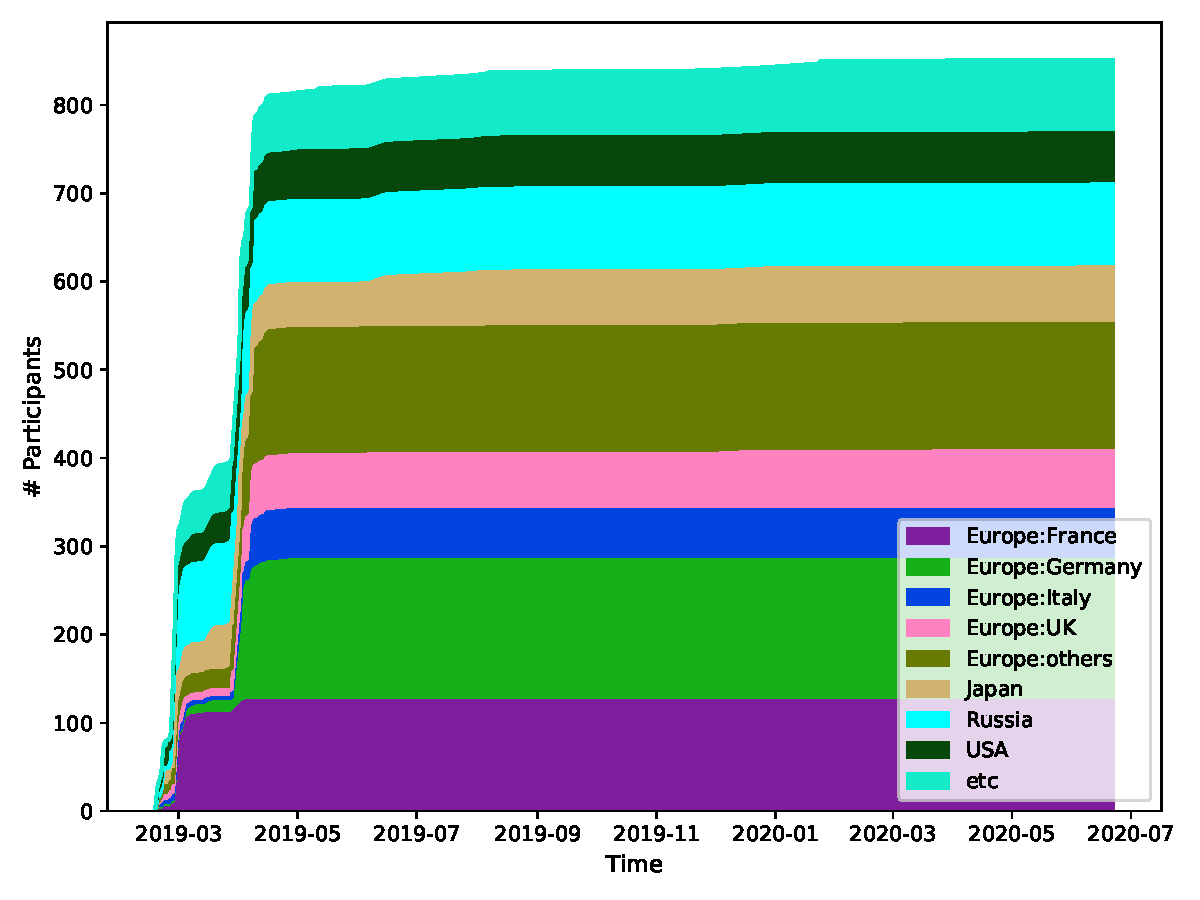
\includegraphics[width=12cm]{../pdfs/TimeSeries.pdf}
\caption{Time series}
\label{fig:timeseries}
\end{center}
\end{figure}
